\documentclass[twocolumn,a4paper]{article}
\usepackage[utf8]{inputenc}
\usepackage[T1]{fontenc}
\usepackage{amsmath}
\usepackage{amssymb}
\usepackage{graphicx}

\usepackage[margin=1cm]{geometry}

\author{Josh Pattman}
\title{Evolutionary Learning In Grouped Gene Networks}
\begin{document}
	\maketitle
    \section{Introduction 1.5pg}
    \begin{itemize}
        \item The displayed genes of a creature, their phenotype, is not only influenced by their own genetic code, know as their genotype, but also through complex interactions between the genes of that creature.
        \item This means that each trait displayed by a creature is actually the result of the entire genotype, and not just a single locus in the genetic code.
        \item The interactions between the different genes is called the gene regulation network.
        \item During evolution, no only are the genes themselves evolving, but the gene regulation network is also evolving.
        \item The evolution of the gene regulatory network can be the cause of patterns in covarying genes emerging, where multiple genes may increase the likelihood of a particular trait being displayed.
        \item More importantly, previously expressed phenotypic patterns may be more likely to be expressed in the future.
    \end{itemize}

    \section{Experiment Setup}
    \begin{itemize}
        \item What you evolved including:
        \item \begin{itemize}
            \item How you represented individuals
            \item What fitness function did you define
            \item What kind of GA you used
            \item Steady state/ generational?  Tournament selection/ fitness proportionate (roulette wheel)?
            \item What kind of crossover (if any) you used.
            \item All parameters (enough detail so a reader could re-implement the GA)
        \end{itemize}
    \end{itemize}

    \section{Reimplemented Results 1pg}
    \begin{figure}[h]
        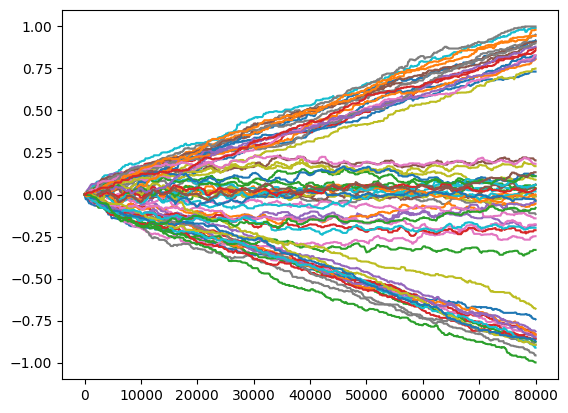
\includegraphics[width=0.48\linewidth]{img/fig2a.png}
        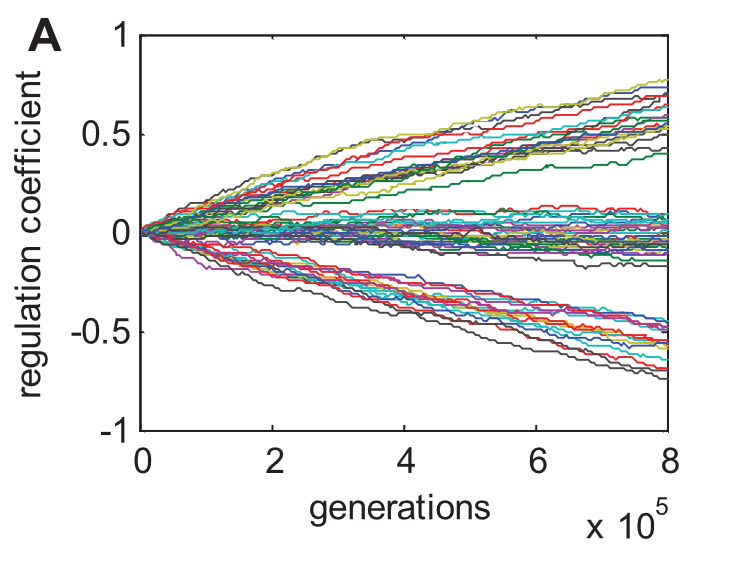
\includegraphics[width=0.48\linewidth]{orig_img/fig2a.png}
        \caption{On the left, the origina paper. On the right, the reimplemented results.}
    \end{figure}

    \begin{figure}[h]
        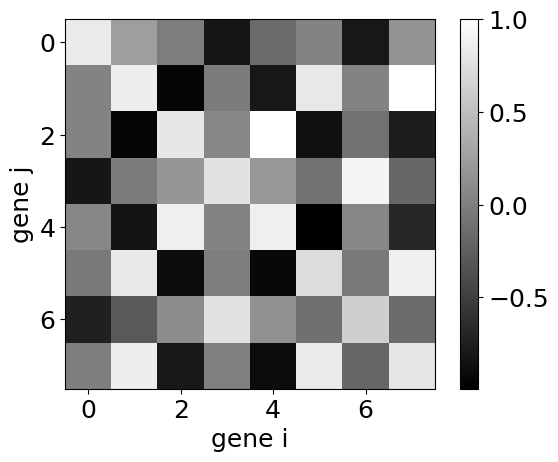
\includegraphics[width=0.48\linewidth]{img/fig2b.png}
        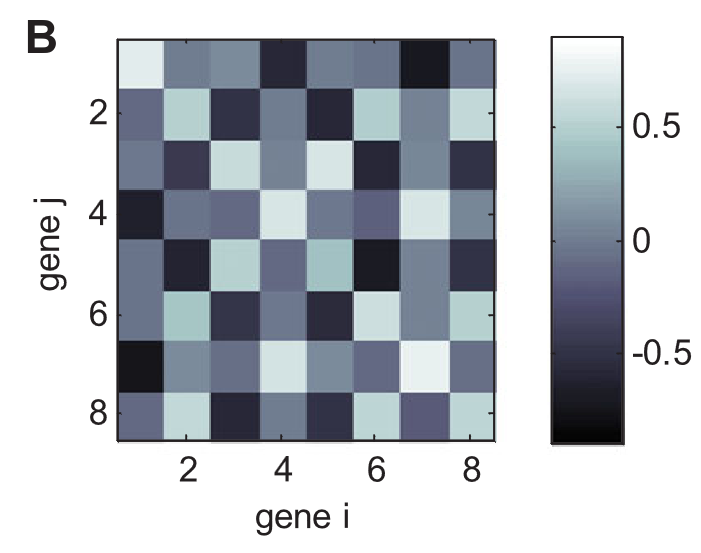
\includegraphics[width=0.48\linewidth]{orig_img/fig2b.png}
        \caption{On the left, the origina paper. On the right, the reimplemented results.}
    \end{figure}

    \begin{figure}[h]
        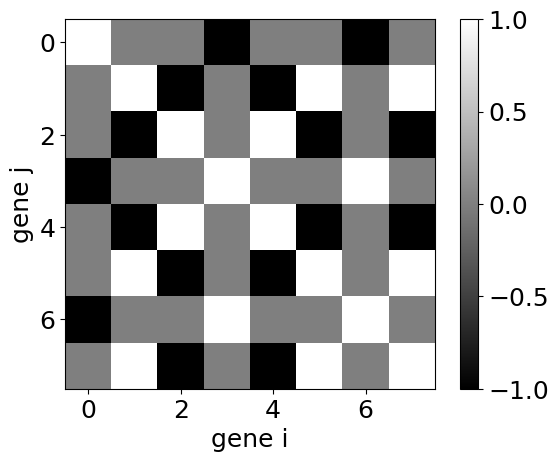
\includegraphics[width=0.48\linewidth]{img/fig2c.png}
        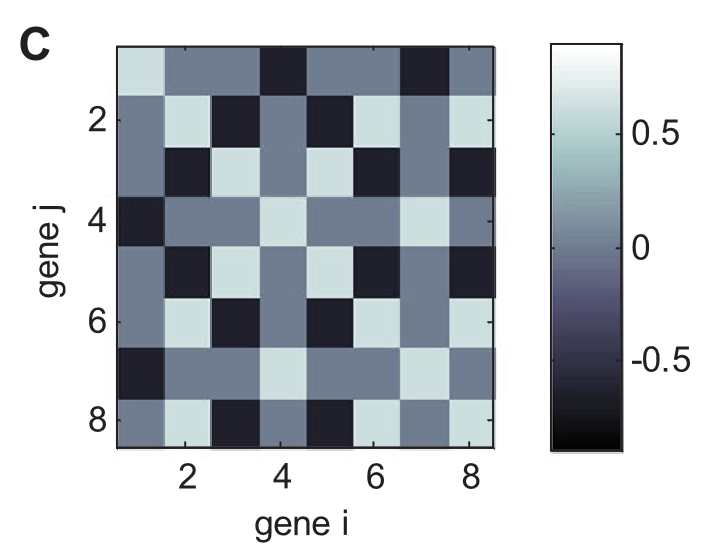
\includegraphics[width=0.48\linewidth]{orig_img/fig2c.png}
        \caption{On the left, the origina paper. On the right, the reimplemented results.}
    \end{figure}

    \begin{figure}[h]
        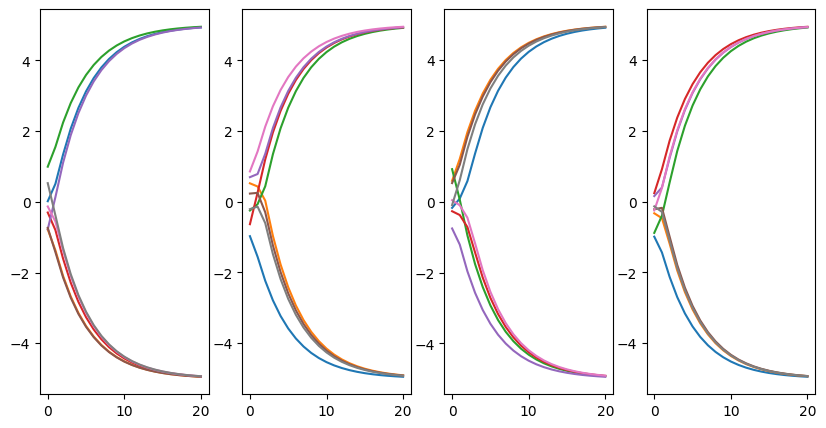
\includegraphics[width=0.9\linewidth]{img/fig2d.png}
        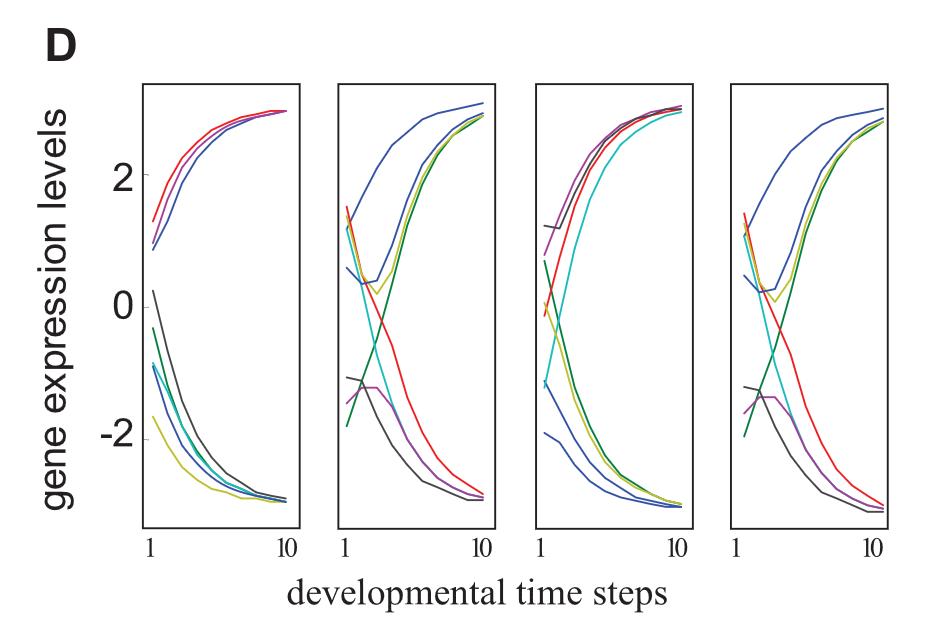
\includegraphics[width=0.9\linewidth]{orig_img/fig2d.png}
        \caption{On the left, the origina paper. On the right, the reimplemented results.}
    \end{figure}

    \begin{figure}[h]
        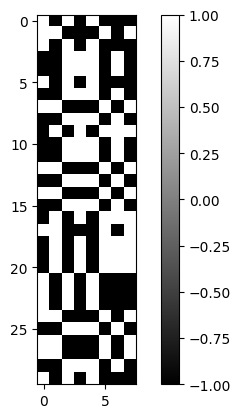
\includegraphics[width=0.45\linewidth]{img/fig2e.png}
        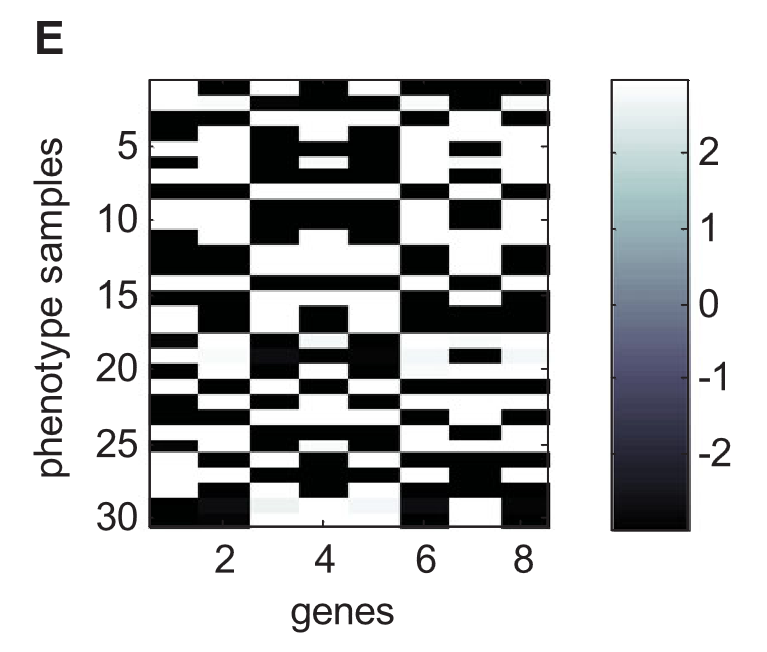
\includegraphics[width=0.45\linewidth]{orig_img/fig2e.png}
        \caption{On the left, the origina paper. On the right, the reimplemented results.}
    \end{figure}

    \begin{itemize}
        \item 1 Page
        \item The reimplemented figures (side by side with the originals)
        \item Discussion of what the results show/don't show, what worked/didn't work, what you learned
    \end{itemize}
    \section{Extension 1pg}
    The previously described model of a GRN is a significant abstraction of the true complexity of the interactions between genes. To extend this work, this paper proposes a more advanced model of a GRN which takes inspiration from protein production in genes.

    In a biological GRN, the expression level of a gene is affected not directly by the expression levels of other genes, but instead by the levels of protiens produced by those genes. It also may be the case that there are significantly fewer unique protiens available for this purpose than there are genes, meaning that genes with similar functions may have to evolve to use similar proteins for regulation. These features of GRNs are not caputered by using a single regulation matrix to represent the interaction between genes.

    \subsection{Goals and Hypothesis}
    This extension focusses on simulating these intermediate messenger proteins in a simplified manner while maintaining maximum similarity with the previously described method, enabling simple comparisons between the two.

    The hypothesis of this experiment is two-fold:
    \begin{enumerate}
        \item \textbf{The gene regulation network will be able to remember previously expressed phenotipic patterns even with an overall reduction in the number of parameters when compared to a dense network.} This is because in the datasets used for these experiments, and indeed real life, there are patterns that the network should be ableto encode into a single protien. Each pattern may then also affect multiple genes in a similar way. These features leave much room for the network to genralise and group certain features that behave in similar ways together.
        \item \textbf{The gene regulation network may become more robust and better at genralising to new patterns, as it is forced to 'make sense' of the input genotype.} In traditional machine learning, a bottleneck is a point in a model where there are fewer features than there were inputs to the model, forcing the network to learn the patterns in its data rather than memerising it. Hypothetically, this should also apply to a GRN with fewer chemicals than genes, as the GRN will need to extract only the most important information from the inputs in order to best create an accurate output.
    \end{enumerate}

    \subsection{Model}
    To represent this new model of a GRN, the interaction matrix must be replaced by two distinct matricies, one for encoding a state of the GRN into a vector representing the protein production, $B_e$, and one for decoding a protien production vector into the updates to each state, $B_d$. Given a number of available proteins $n_{protein}$ and the genotype size $n_{genotype}$, $B_e$ has dimensions $(n_{protein},n_{genotype})$, and $B_d$ has dimensions $(n_{genotype},n_{protein})$. Given these matricies the phenotype at the next timestep, column vector $P(t+1)$, is given by the equation
    \begin{equation}
        P(t+1) = P(t) + \tau_1 \sigma (B_d (B_e P(t))) - \tau_2 P(t)
    \end{equation}
    Where $\tau_1$ and $\tau_2$ are the update rate and decay rate of the network respectively, and $\sigma$ is the sigmoid function.

    This method has some useful properties aside from furfilling the aim to simulate the intermediate properties:
    \begin{enumerate}
        \item Mapping the previous state to the next state with two matricies may be a faster computation with fewer parameters compared to a single interaction matrix, as long as
        \begin{equation}
            n_{protien} < n_{genotype} \div 2
        \end{equation}
            
        \item As the matricies are multiplied linearly together, it is possible to find the equivalent single interaction matrix by performing the calculation
        \begin{equation}
            B = B_dB_e
        \end{equation}
        Computing the single interaction matrix enables easy comparison to both the original approach, and the weights derived from Hebbs rule, which is useful when evaluating if this model maintains the tendancy to move towards the Hebbian weights.
    \end{enumerate}
    \begin{itemize}
        \item TODO: Support the value of asking that question (using literature)
    \end{itemize}


    \section{Extension Results}
    \begin{itemize}
        \item 1.5 page
    \end{itemize}


    \section{Conclusion}
    \begin{itemize}
        \item one page
        \item What do you conclude from that
        \item significance of the extension results
        \item critique/evaluation
    \end{itemize}


    \section{Appendix}


\end{document}